 \documentclass{beamer}
%
% Choose how your presentation looks.
% For more themes, color themes and font themes, see:
% http://deic.uab.es/~iblanes/beamer_gallery/index_by_theme.html
%
\mode<presentation>
{
  \usetheme{Madrid}      % or try Darmstadt, Madrid, Warsaw, ...
  \usecolortheme{seahorse} % or try albatross, beaver, crane, ...
  \usefonttheme{serif}  % or try serif, structurebold, ...
  \setbeamertemplate{navigation symbols}{}
  \setbeamertemplate{caption}[numbered]
  \setbeamertemplate{itemize/enumerate body begin}{\large}
\setbeamertemplate{itemize/enumerate subbody begin}{\large}
\setbeamertemplate{itemize/enumerate subsubbody begin}{\large}

  \usepackage{amsmath}
  \usepackage{bm} 
  \usepackage{subcaption}
  \usepackage{tcolorbox}
  \usepackage[export]{adjustbox}
  \tcbuselibrary{most}
  \usepackage{arydshln}
  \usepackage{tikz}
  \usetikzlibrary{plotmarks}
  \usepackage{pgfplots}
  \usepackage{booktabs}
 %\usepackage{enumitem}
%\usepackage{enumerate}
  %\usepackage[shortlabels]{enumitem}
} 


\definecolor{myblue}{RGB}{65,105,225} 
\definecolor{myorange}{RGB}{250,190,0}

\setbeamercolor{structure}{fg=white,bg=myorange}
\setbeamercolor*{palette primary}{fg=myblue,bg=myorange}
\setbeamercolor*{palette secondary}{fg=white,bg=myblue}
\setbeamercolor*{palette tertiary}{bg=myblue,fg=white}
\setbeamercolor*{palette quaternary}{fg=white,bg=myorange!50}

\setbeamercolor{frametitle}{fg=black!90!myblue}

\setbeamercolor{section in head/foot}{fg=white,bg=myblue}
\setbeamercolor{author in head/foot}{fg=black,bg=myorange}
\setbeamercolor{title in head/foot}{fg=white,bg=myblue}

\setbeamertemplate{navigation symbols}{}

\setbeamertemplate{itemize/enumerate body begin}{\large}
\setbeamertemplate{itemize/enumerate subbody begin}{\large}


\defbeamertemplate*{headline}{mytheme}
{%
  \begin{beamercolorbox}[ht=2.25ex,dp=3.75ex]{section in head/foot}
    \insertnavigation{\paperwidth}
  \end{beamercolorbox}%
}%

\defbeamertemplate*{footline}{mytheme}
{
  \leavevmode%
  \hbox{%
  \begin{beamercolorbox}[wd=.5\paperwidth,ht=2.25ex,dp=1ex,right]{author in head/foot}%
    \usebeamerfont{author in head/foot}\insertshortauthor\hspace*{2em}
  \end{beamercolorbox}%
  \begin{beamercolorbox}[wd=.5\paperwidth,ht=2.25ex,dp=1ex,left]{title in head/foot}%
    \usebeamerfont{title in head/foot}\hspace*{2em}\insertshortsubtitle\hspace*{2em}
    \insertframenumber{} / \inserttotalframenumber
  \end{beamercolorbox}}%
  \vskip0pt%
}

\usepackage[english]{babel}
%\usepackage[utf8x]{inputenc}
\usepackage{xcolor}
\usepackage{listings}
\usepackage{pgf}  
\usepackage{textpos}
\usepackage{tabulary}
\usepackage{scrextend}
\usepackage{hyperref}
\usepackage{setspace}
\usepackage{rotating}
\lstset
{
    language=[LaTeX]TeX,
    breaklines=true,
    basicstyle=\tt\scriptsize,
    %commentstyle=\color{green}
    keywordstyle=\color{blue},
    %stringstyle=\color{black}
    identifierstyle=\color{magenta},
}
\newcommand{\bftt}[1]{\textbf{\texttt{#1}}}
%\newcommand{\comment}[1]{{\color[HTML]{008080}\textit{\textbf{\texttt{#1}}}}}
\newcommand{\cmd}[1]{{\color[HTML]{008000}\bftt{#1}}}
\newcommand{\bs}{\char`\\}
\newcommand{\cmdbs}[1]{\cmd{\bs#1}}
\newcommand{\lcb}{\char '173}
\newcommand{\rcb}{\char '175}
\newcommand{\cmdbegin}[1]{\cmdbs{begin\lcb}\bftt{#1}\cmd{\rcb}}
\newcommand{\cmdend}[1]{\cmdbs{end\lcb}\bftt{#1}\cmd{\rcb}}

\newcommand{\wllogo}{\textbf{Overleaf}}

% this is where the example source files are loaded from
% do not include a trailing slash
\newcommand{\fileuri}{https://raw.githubusercontent.com/GiancarloSucci/UniBo.IDSEPC.A2022/main/A2022.IDSEPCLaTeX/}


\usepackage{stackengine}
\def\Ruble{\stackengine{.67ex}{%
  \stackengine{.48ex}{\textsf{P}}{\rule{.8ex}{.12ex}\kern.6ex}{O}{r}{F}{F}{L}%
  }{\rule{.8ex}{.12ex}\kern.6ex}{O}{r}{F}{F}{L}\kern-.1ex}



%----------------------------------------------------------------------------------------
%	TITLE PAGE
%----------------------------------------------------------------------------------------
\title[L07]{Artificial Intelligence, Blockchain, e Criptovalute nello Sviluppo Software \newline\newline
Lezione 7: Drawing as a Cognitive Experience (for SW Development)} % The short title appears at the bottom of every slide, the full title is only on the title page

\author[{\tiny Giancarlo Succi }]{Giancarlo Succi\\\\ Dipartimento di Informatica -- Scienza e Ingegneria\\Universit\`{a} di Bologna\\
\bftt{g.succi@unibo.it}
} % Your name
\institute[unibo] % Your institution as it will appear on the bottom of every slide, may be shorthand to save space


\date{} % Date, can be changed to a custom date

\setbeamertemplate{navigation symbols}{}
\AtBeginSection[]
{
        \begin{frame}<beamer>{Outline}
                \tableofcontents[currentsection]
        \end{frame}
}
\begin{document}

\begin{frame}
\titlepage % Print the title page as the first slide

\end{frame}

%=============================================

\addtobeamertemplate{frametitle}{}{%
\begin{textblock*}{10mm}(-0.01mm,-0.95cm)
\includegraphics[width=0.9cm]{unibo-logo.png}
\end{textblock*}}

%=============================================


\begin{frame}
{\centerline{Structure of the lecture}}
\begin{itemize}
    \item Understanding ourselves and the others
    \item Drawing
    \item Mental states while drawing
    \item Processes in drawing and in software
    \end{itemize}
\end{frame}

\begin{frame}
{\centerline{Understanding ourselves and the others}}
 
\begin{itemize}
\item Software is centered in the mind
\begin{itemize}
\item The mind of developers, managers, customers, etc
\end{itemize} 
\item Indeed, it is therefore essential to understand the minds
\begin{itemize}
\item Ours and the one of the people around us
\end{itemize} 
\item We often resort to drawing to help structuring our thoughts
\begin{itemize}
\item And likewise do the people around us
\end{itemize} 
\item We now therefore turn our attention to understanding \textcolor{red}{the role of \textbf{drawing} in developing \textbf{software}}
\end{itemize} 

\end{frame}

\begin{frame}
{\centerline{The approach of this lecture}}
 
\begin{itemize}
\item We will use one of the several existing approaches, focusing on the work of Freud, through the analysis of Gianluca Solla in the book ``Disegnare, la formula di Freud,'' published by Orthotes in 2022
\item We will consider Freud both as:
\begin{itemize}
\item a researcher, explaining the meaning of drawing
\item a (very primitive) artist, that expresses his feelings in drawing
\end{itemize} 
\item In this way, we will attempt to grasp a bit of the intrinsic meaning of drawing:
\begin{itemize}
\item why it is so relevant to software engineering
\begin{itemize}
\item and so why Freud is a software engineer and we are psychoanalysts ...
\end{itemize} 
\item the way it is ontologically a wicked problem
\end{itemize} 
\end{itemize} 

\end{frame}



\begin{frame}
{\centerline{A spot in a letter}}
 
\begin{itemize}
    \item Freud writing a letter to his girlfriend Martha in 1882:
\end{itemize} 

\begin{center}
 \includegraphics[width=6cm]{P2023.AIBCCSS.Drawing/LetterFreudGirlfriend.png}
 
 \end{center}
 
\begin{itemize}
    \item In an earlier mail: ``Give an artistic shape to the experience.''
\end{itemize} 

\begin{center}
\tiny
Source of the content: Gianluca Solla ``Disegnare, la formula di Freud,'' Orthotes, 2022, page 7.
\end{center}
\end{frame}

\begin{frame}
{\centerline{Interpreting}}
 
\begin{itemize}
    \item \textcolor{red}{Give} an \textcolor{blue}{artistic} \textcolor{orange}{shape} to the \textcolor{cyan}{experience} \newline
\begin{itemize}
    \item \textcolor{cyan}{\bf Experience}: the core, but alone remains meaningless and vanishes\newline
    \item \textcolor{orange}{\bf Shape}: the interpretation of to the experience \newline
    \item \textcolor{blue}{\bf Artistic}: the form and the technological ability underlying the creation of the shape\newline
    \item \textcolor{red}{\bf Give}: we, as subjects, creating such artistic interpretation\newline
\end{itemize} 
\end{itemize} 

\begin{center}
\tiny
Source of the content: Gianluca Solla ``Disegnare, la formula di Freud,'' Orthotes, 2022.
\end{center}
\end{frame}

\begin{frame}
{\centerline{The role of the spot}}
 
\begin{itemize}
    \item The random spot starts having a meaning
    \item This is at the core of the problem: what is the process by which we give meaning to elements
    \item The meaning may be the result of a a random, non linear, non consequential sequence of actions
    \item The meaning of the spot may evolve in time -- just think at how it started
    \item And our problem is how we integrate such meaning into the big picture
\end{itemize} 

\begin{center}
\tiny
Source of the content: Gianluca Solla ``Disegnare, la formula di Freud,'' Orthotes, 2022.
\end{center}
\end{frame}

\begin{frame}
{\centerline{Drawing}}
 
\begin{itemize}
    \item Drawing is how we give meaning to spots
    \item Drawing has two very important roles:
 \begin{itemize}
    \item  The resulting picture
    \item The process of drawing, which is a way in which we perceive the reasoning behind
 \begin{itemize}
    \item  Drawing has a strong relevance as drawing beyond the resulting picture
    \end{itemize} 
\end{itemize} 
 \end{itemize} 


\begin{center}
\tiny
Source of the content: Gianluca Solla ``Disegnare, la formula di Freud,'' Orthotes, 2022.
\end{center}
\end{frame}

\begin{frame}
{\centerline{Kind of Drawings}}
 
\begin{itemize}
    \item Drawing to \textcolor{red}{schematize a concept}
    \begin{itemize}
    \item Simplifications of what is in the mind
   \end{itemize}
    \item Drawing to \textcolor{blue}{present an experience}
    \begin{itemize}
    \item Narration of what is in the mind
   \end{itemize}
   \item The two purposes are strictly interconnected and think at software:
       \begin{itemize}
           \item \textcolor{red}{Class diagrams}, schematizing a concept
    	\item \textcolor{blue}{User stories}, presenting a experience
   \end{itemize}
   \item And in both cases, drawing is a way to objectify what is in the mind
 \end{itemize} 


\begin{center}
\tiny
Source of the content: Gianluca Solla ``Disegnare, la formula di Freud,'' Orthotes, 2022.
\end{center}
\end{frame}

\begin{frame}
{\centerline{Understanding the Drawings (1/2)}}
 
\begin{itemize}
   \item Drawings are starting point for an introspection in the (distributed) mind of the author(s)
\begin{itemize}
   \item They also present the reasoning process
 \end{itemize} 
      \item Drawings are bridges from the (past) history to the (future) desires or fears
 \item As such, using our schema of tame vs. wicked processes,
 \begin{itemize}
   \item  drawing is the wicked process of the self-exploration of the mind
  \begin{itemize}
   \item while drawing we understand the drawing and refine it, stroke after stroke
   \item the timing of drawing play a major role
    \end{itemize} 
      \end{itemize} 

 \end{itemize} 

\begin{center}
\tiny
Source of the content: Gianluca Solla ``Disegnare, la formula di Freud,'' Orthotes, 2022.
\end{center}
\end{frame}

\begin{frame}
{\centerline{Understanding the Drawings (2/2)}}
 
\begin{itemize}
  \item and $\ldots{}$
\begin{itemize}
     \item understanding the drawing is a ``double wicked'' process of exploring such inner exploration and
     \item its time evolution
\end{itemize}
 \item Using the words of Freud:
 \begin{itemize}
   \item Phantasieren, \"{U}bersetzen, Erraten 
    \begin{itemize}
   \item Fantasizing, translating, wandering, often (but not always) as when are schematizing a concept and then
    \end{itemize} 
   \item Speculieren, Theorisieren, Phantasieren
   \begin{itemize}
   	\item Thinking, theorizing, fantasizing, often (but not always) as when we are presenting a experience
    \end{itemize} 
 \end{itemize} 
 \end{itemize} 

\begin{center}
\tiny
Source of the content: Gianluca Solla ``Disegnare, la formula di Freud,'' Orthotes, 2022.
\end{center}
\end{frame}



\begin{frame}
{\centerline{Phantasieren (fantasizing) (1/3)}}
 
\begin{itemize}
   \item Two roots from Latin:
\begin{itemize}
   \item \textcolor{red}{Fantasy}, imagination
   \begin{itemize}
   \item Referring to the creative act of the mind to think at entities, sometimes not yet existing in the reality
    \end{itemize} 
   \item \textcolor{blue}{Phantom}, ghost
      \begin{itemize}
   \item Referring to the ability of following the mind into their deep thoughts, reflections, spanning also to the subconcious
    \end{itemize} 
 \end{itemize} 
  \end{itemize} 

\begin{center}
\tiny
Source of the content: Gianluca Solla ``Disegnare, la formula di Freud,'' Orthotes, 2022.
\end{center}
\end{frame}


\begin{frame}
{\centerline{Phantasieren (fantasizing) (2/3)}}
 
\begin{itemize}
 \item As already pointed out for the model of the dual mind, the researcher must go beyond the ``standard'' experimental practices
       \begin{itemize}
   \item For the model of the mind, we referred to the \textcolor{red}{ethnographic exploration}
   \item In this case, our ``ethnography'' will refer to the mental exploration of the mind -- we could even say that the researcher or the software engineering is engaged in a \textcolor{red}{psychoanalytical exploration} of the mind
       \end{itemize} 
   \item This is not \textbf{anyhow} referred to any therapeutic initiative
 \end{itemize} 
 
\begin{center}
\tiny
Source of the content: Gianluca Solla ``Disegnare, la formula di Freud,'' Orthotes, 2022.
\end{center}
\end{frame}

\begin{frame}
{\centerline{Phantasieren (fantasizing) (3/3)}}
 
\begin{itemize}
   \item However, also from a purely technical perspective, \textcolor{red}{none would be able to understand} the requirements and the requests of colleagues, managers, employees, or customers   
      \begin{itemize}
             \item \textcolor{red}{unless there is deep exploration} and understanding of the \textcolor{orange}{\bf mind} in its fantasizing
    \end{itemize} 
 \item Something to keep well in mind:
 \begin{itemize}
 \item This is not:
  \begin{itemize}
  \item less rigorous
  \item less technical
  \item less difficult
  \item less related to software engineering
 \end{itemize} 
   than writing a highly complex piece of C++ code for a new device driver
 \end{itemize} 
 \end{itemize} 
 
\begin{center}
\tiny
Source of the content: Gianluca Solla ``Disegnare, la formula di Freud,'' Orthotes, 2022.
\end{center}
\end{frame}

\begin{frame}
{\centerline{Decoding the drawing (1/3)}}
 
\begin{itemize}
   \item Drawing defines a language to interpret
   \item The interpretation involves
   \begin{itemize}
   \item The individual elements
   \item The drawing as a whole
   \item The temporal placement of each individual stroke
\end{itemize} 
  \item However, the language is not defined by the strokes in the resulting picture, which are in constant evolution, not static:
     \begin{itemize}
   \item Therefore, it is a language that can be hardly formalized
   \item This is why, for instance, the structure of a code repository cannot be explained without looking at its time evolution
\end{itemize} 
\item It has a role per-se, beyond what we can na\"{i}vely think that it represent
 \end{itemize} 

\begin{center}
\tiny
Source of the content: Gianluca Solla ``Disegnare, la formula di Freud,'' Orthotes, 2022.
\end{center}
\end{frame}

\begin{frame}
{\centerline{Modeling the time evolution of a code repository}}

\begin{center}
 \includegraphics[width=8cm]{P2023.AIBCCSS.Drawing/Lagrein.jpg}
 
 \end{center}

\begin{center}
\tiny
Source of the picture: Andrejs Jermakovics, Raimund Moser, Alberto Sillitti, and Giancarlo Succi. Visualizing Software Evolution with Lagrein. In Companion to the 23rd ACM SIGPLAN Conference on Object-Oriented Programming Systems Languages and Applications, OOPSLA Companion ’08. ACM, October 2008, page 750.
\end{center}
\end{frame}

\begin{frame}
{\centerline{Decoding the drawing (2/3)}}
 
\begin{itemize}
   \item How Freud represented such dynamic associations
 \end{itemize} 

\begin{center}
 \includegraphics[width=10cm]{P2023.AIBCCSS.Drawing/aphasien.jpg}
 
 \end{center}

\begin{center}
\tiny
Source of the content: Gianluca Solla ``Disegnare, la formula di Freud,'' Orthotes, 2022; Sigmund Freud ``Zur Auffassung der Aphasien. Eine kritische Studie,'' Franz Deuticke, 1891, pag. 79, fig. 8.
\end{center}
\end{frame}


\begin{frame}
{\centerline{Decoding the drawing (3/3)}}
 
\begin{center}
 \includegraphics[width=10cm]{P2023.AIBCCSS.Drawing/flowInsideMemory.jpg}
 
 \end{center}
\begin{itemize}
   \item This is how Freud represented the flow of information
\begin{itemize}
   \item W are the neurons connected to perception
   \item Wz are the symbols of how such perception is taken
   \item Ub is the subconscious, as memory traces that are unaccessible to the conscious mind
   \item Vb is the rewriting related to words
 \end{itemize} 
   \item In essence, the physical life is a process
 \end{itemize} 

\begin{center}
\tiny
Source of the content: Gianluca Solla ``Disegnare, la formula di Freud,'' Orthotes, 2022, the pictures comes from page 23 and it is allegedly taken from Sigmund Freud, Briefe and Wilhelm Flie\ss. 1887-1904, S. Fischer, Frankfurt a.M., 1994
\end{center}
\end{frame}

\begin{frame}
{\centerline{Reflecting on the drawings}}
\begin{itemize}
   \item Drawing also evidences what is missing
   \item Indeed, drawing has limitations, Freud defines it a ``Hilfsapparat"
   \begin{itemize}
   \item but still it is essential
   \end{itemize} 
   \item It helps also as evidencing the time-variant nature of the mind as a collection of differences 
      \begin{itemize}
   \item and any representation is in itself a very limited perspective
   \item as it is well evidences considering the structure of a software repository
   \end{itemize} 
 \end{itemize} 

\begin{center}
\tiny
Source of the content: Gianluca Solla ``Disegnare, la formula di Freud,'' Orthotes, 2022
\end{center}
\end{frame}

\begin{frame}
{\centerline{Sample time evolution of a code repository}}

\begin{center}
 \includegraphics[width=12cm]{P2023.AIBCCSS.Drawing/issuesArrivals.jpg}
 
 \end{center}

\begin{center}
\tiny
Source of the picture: Vladimir Ivanov, Alexey Reznik, and Giancarlo Succi. ``Comparing the reliability of software systems: A case study on mobile operating systems.'' Information Sciences. Elsevier,  2018, 423:398-411, fig. 1, page 405.
\end{center}
\end{frame}

\begin{frame}
{\centerline{Moving on}}
\begin{itemize}
   \item Nature of wicked problems:
      \begin{itemize}
   \item Freud: ``We should be almost ashamed that after so much work we find always new difficulties in understanding the fundamental facts that are in front of us"
   \end{itemize} 
   \item It is always in a unstable balance between invention and repetition
   \item Every end is always like a new beginning
   \item This is why Freud represent his medical experiences, the ``Clinical Cases'' as a storyteller
    \begin{itemize}
   \item We will discuss more about storytelling later on
   \end{itemize} 
  \item We will now have a review of a few drawings of Freud as per the reference book, to see how their interpretation can help explaining how to interpret drawings in software development
 \end{itemize} 

\begin{center}
\tiny
Source of the content: Gianluca Solla ``Disegnare, la formula di Freud,'' Orthotes, 2022, the citation of Freud is allegedly from Sigmund Freud ``Hemmung, Symptom und Angst,'' 1926.
\end{center}
\end{frame}


\begin{frame}
{\centerline{Drawings in Trieste (1/2)}}

\begin{itemize}
   \item Drawing to select elements for further analysis
 \end{itemize} 


\begin{center}
 \includegraphics[width=6cm]{P2023.AIBCCSS.Drawing/selectingElementsFreud.jpg}
 
 \end{center}

\begin{center}
\tiny
Source of the content: Gianluca Solla ``Disegnare, la formula di Freud,'' Orthotes, 2022, pag. 39
\end{center}
\end{frame}

\begin{frame}
{\centerline{Drawings in Trieste (2/2)}}

\begin{itemize}
   \item Drawing to describe the own experience in terms of the perception of the outer world
 \end{itemize} 


\begin{center}
 \includegraphics[width=5.5cm]{P2023.AIBCCSS.Drawing/outerWorld.jpg}
 
 \end{center}

\begin{itemize}
   \item Here we perceive how the drawing defines a wicked problem, where a solution is the beginning of a new investigation.
 \end{itemize} 

\begin{center}
\tiny
Source of the content: Gianluca Solla ``Disegnare, la formula di Freud,'' Orthotes, 2022, pag. 38
\end{center}
\end{frame}

\begin{frame}
{\centerline{Drawing in a letter to Wilhelm (1/2)}}

\begin{itemize}
   \item Drawing to describe a model that has been devised
 \end{itemize} 


\begin{center}
 \includegraphics[width=3.5cm]{P2023.AIBCCSS.Drawing/schematizzazione.jpg}
 
 \end{center}

\begin{itemize}
   \item We notice here a completely different approach to draw, where there is quite a statement of correctness
 \end{itemize} 

\begin{center}
\tiny
Sources of the content: Gianluca Solla ``Disegnare, la formula di Freud,'' Orthotes, 2022, pag. 74
\end{center}
\end{frame}

\begin{frame}
{\centerline{Drawing in a letter to Wilhelm (2/2)}}

\begin{itemize}
   \item But look at how he got there:
 \end{itemize} 


\begin{center}
 \includegraphics[width=5cm]{P2023.AIBCCSS.Drawing/towardBuildingASchema.jpg}
 
 \end{center}


\begin{center}
\tiny
Source of the content: Gianluca Solla ``Disegnare, la formula di Freud,'' Orthotes, 2022, pag. 51
\end{center}
\end{frame}

\begin{frame}
{\centerline{``The psyche is extended. Knows nothing about it''}}
\begin{itemize}
\item This is an intuition of Freud, connected to our discussion of the extended mind, which is triggered by this drawing:
\begin{itemize}
\item P(erception), M(otility), Inc(onscious), Pre(conscious), Mn(estic traces)
 \end{itemize}
  \end{itemize} 

\begin{center}
 \includegraphics[width=10cm]{P2023.AIBCCSS.Drawing/perceptionMotility.jpg}
 
 \end{center}


\begin{center}
\tiny
Source of the content: Gianluca Solla ``Disegnare, la formula di Freud,'' Orthotes, 2022, pag. 74.
\end{center}
\end{frame}


\begin{frame}
{\centerline{From drawing to understanding}}
\begin{itemize}
\item All this works of Freud on drawings for us is interesting under a dual perspective:
\begin{itemize}
\item For what we said, since through pictures we understand the minds of the people we are dealing with
\item Because Freud itself, despite being a neurologist, so full aware of how the brain works, preferred drawing to elaborate ideas on the work of the mind:
\begin{itemize}
\item they are more relevant than the physiological analysis;
\item \textit{``individuals and interactions over processes and tools.''}
 \end{itemize} 
 \end{itemize} 
 \end{itemize} 

\begin{center}
\tiny
Source of the content: Gianluca Solla ``Disegnare, la formula di Freud,'' Orthotes, 2022.
\end{center}
\end{frame}

\begin{frame}
{\centerline{Drawing and Coding}}
\begin{itemize}
\item We end this lecture discussing the similarities in the brain activity between coding and drawing, a further reinforcement of the relevance of drawings in our work.
\item We have run an experiment with 22 participants coding and sketching
\item The participants were first instructed and then had a sessions in which they prepared for recoding, and they they were given a task to solve.
\item The data has been collected using a 32-channels portable EEG cap.
\end{itemize} 

\begin{center}
\tiny
Source of the content: Gcinizwe Dlamini, Giancarlo Succi, Nataliya Tupikina ``Is the mind of a software developer similar to that of an artist? Focus on drawing,'' Under review, 2023.
\end{center}
\end{frame}

\begin{frame}
{\centerline{Drawing and Coding -- Results (1/2)}}

 \begin{itemize}
\item Clusters of values of  $\alpha/\beta$ and $\theta/\alpha$ when resting (the red \textcolor{red}{$\times$}), programming (the blue \textcolor{blue}{$\bullet$}), and drawing a picture (the olive
    \textcolor{olive}{$\bm{+}$})
  \end{itemize} 

\begin{figure}[!ht]
    \centering
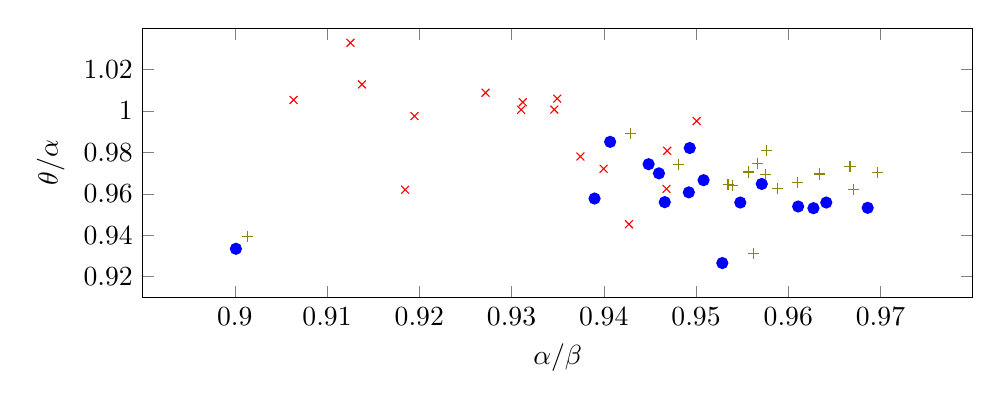
\begin{tikzpicture}
  \begin{axis}[
        width=\linewidth,
        height=5cm,
        xmin=0.89,xmax=0.98,ymin=0.91,ymax=1.04,
        xlabel={$\alpha/\beta$},
        ylabel={$\theta/\alpha$},
        xtick={0.90,0.91,...,0.97},
        ytick={0.92,0.94,...,1.02}
        ]
%       \node[text=blue,font=\sffamily\bfseries,scale=2] at (3,70) {X};
       \addplot+[blue,only marks,mark=*, samples=16,mark
        options={fill=blue}] coordinates {
            (	0.94932	,	0.98214	)
            (	0.96273	,	0.95309	)
            (	0.96107	,	0.95390	)
            (	0.90012	,	0.93347	)
            (	0.94922	,	0.96073	)
            (	0.96861	,	0.95327	)
            (	0.93900	,	0.95774	)
            (	0.94069	,	0.98512	)
            (	0.94486	,	0.97434	)
            (	0.95480	,	0.95581	)
            (	0.94661	,	0.95600	)
            (	0.95082	,	0.96662	)
            (	0.94598	,	0.96991	)
            (	0.95285	,	0.92659	)
            (	0.95713	,	0.96479	)
            (	0.96412	,	0.95582	)
            } node[above,pos=.57,blue] {};

\addplot+[olive,only marks,mark=+, samples=16,mark
            options={fill=olive}] coordinates {
(0.95764,0.98103) (0.96709,0.96201) (0.96341,0.96958) (0.90135,0.93923) (0.95749,0.96918) (0.96969,0.97018) (0.95397,0.96424) (0.94288,0.98905) (0.94813,0.97418) (0.95887,0.96270) (0.95347,0.96450) (0.95568,0.97055) (0.95662,0.97482) (0.95626,0.93122) (0.96669,0.97311) (0.96096,0.96567)
            } node[above,pos=.57,olive] {};

\addplot+[red,only marks,mark=x, samples=16,mark
            options={fill=red}] coordinates {
    (	0.90637	,	1.00536	)
    (	0.93464	,	1.00072	)
    (	0.95007	,	0.99515	)
    (	0.91846	,	0.96201	)
    (	0.93747	,	0.97805	)
    (	0.93496	,	1.00600	)
    (	0.92718	,	1.00885	)
    (	0.91254	,	1.03297	)
    (	0.93122	,	1.00427	)
    (	0.94688	,	0.98081	)
    (	0.91948	,	0.99758	)
    (	0.91378	,	1.01288	)
    (	0.93104	,	1.00059	)
    (	0.94273	,	0.94534	)
    (	0.93998	,	0.97212	)
    (	0.94680	,	0.96241	)
    
    } node[above,pos=.57,red] {};
%      \node[text=red,scale=2] at (0.931,0.992){\bm{$\bullet$}};


\end{axis}
\end{tikzpicture}
\end{figure}


\begin{center}
\tiny
Source of the content: Gcinizwe Dlamini, Giancarlo Succi, Nataliya Tupikina ``Is the mind of a software developer similar to that of an artist? Focus on drawing,'' Under review, 2023.
\end{center}
\end{frame}

\begin{frame}
{\centerline{Drawing and Coding -- Results (2/2)}}

 \begin{itemize}
\item Empirical distribution functions of (a) $\alpha/\beta$  and (b) $\theta/\alpha$ for resting ($F_r$), programming ($F_p$), and drawing ($F_d$)
  \end{itemize} 

\begin{figure}[!ht]
\centering
\begin{subfigure}{.5\textwidth}
  \centering
    \resizebox{\textwidth}{!}{%
    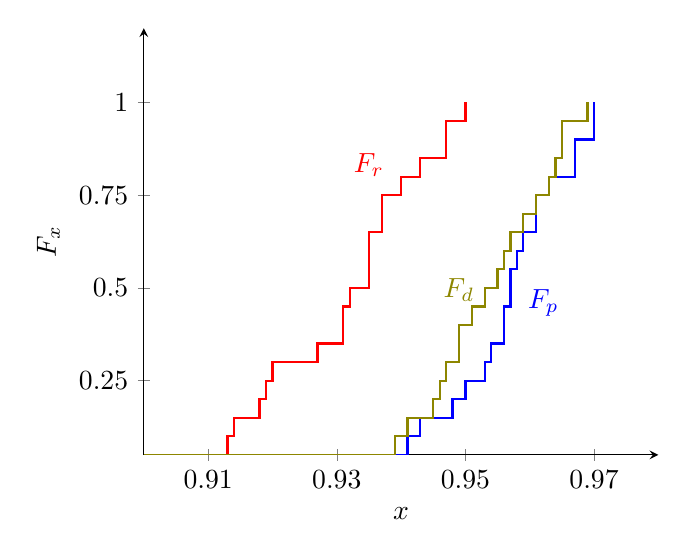
\begin{tikzpicture}
    \begin{axis}[%
        height=7cm,
        xlabel=$x$
        ,ylabel=$F_x$
        ,axis x line = bottom,axis y line = left
        ,ytick={0.25,0.5,...,1}
        ,ymax=1.2 % or enlarge y limits=upper
        ,xmin=0.90
        ,xmax=0.98
        ,xtick={0.91,0.93,...,0.97}
        ]
    \addplot+[red,const plot, no marks, thick] coordinates {(0.906, 0.050) (0.913, 0.100) (0.914, 0.150) (0.918, 0.200) (0.919, 0.250) (0.920, 0.300) (0.927, 0.350) (0.931, 0.400) (0.931, 0.450) (0.932, 0.500) (0.935, 0.550) (0.935, 0.600) (0.935, 0.650) (0.937, 0.700) (0.937, 0.750) (0.940, 0.800) (0.943, 0.850) (0.947, 0.900) (0.947, 0.950) (0.950, 1.000)} node[above=0.85cm, pos=.57,red] {$F_r$};
    
    \addplot+[blue,const plot, no marks, thick] coordinates {(0.901, 0.050) (0.941, 0.100) (0.943, 0.150) (0.948, 0.200) (0.950, 0.250) (0.953, 0.300) (0.954, 0.350) (0.956, 0.400) (0.956, 0.450) (0.957, 0.500) (0.957, 0.550) (0.958, 0.600) (0.959, 0.650) (0.961, 0.700) (0.961, 0.750) (0.963, 0.800) (0.967, 0.850) (0.967, 0.900) (0.970, 0.950) (0.970, 1.000)} node[below=1.2cm,pos=.77,blue] {$F_p$};
    
    \addplot+[olive,const plot, no marks, thick] coordinates {(0.900, 0.050) (0.939, 0.100) (0.941, 0.150) (0.945, 0.200) (0.946, 0.250) (0.947, 0.300) (0.949, 0.350) (0.949, 0.400) (0.951, 0.450) (0.953, 0.500) (0.955, 0.550) (0.956, 0.600) (0.957, 0.650) (0.959, 0.700) (0.961, 0.750) (0.963, 0.800) (0.964, 0.850) (0.965, 0.900) (0.965, 0.950) (0.969, 1.000) } node[above=0.25cm,pos=.36,olive] {$F_d$};
    \end{axis}
    \end{tikzpicture}
    }
    % \caption{\textbf{Empirical distribution functions for resting ($F_r$), programming ($F_p$), and drawing ($F_d$)}}
    % \label{fig:edfThetaAlpha}
% \end{figure}
  \caption{EDF of $\alpha/\beta$}
  \label{fig:sub1}
\end{subfigure}%
\begin{subfigure}{.5\textwidth}
  \centering
    \resizebox{\textwidth}{!}{%
    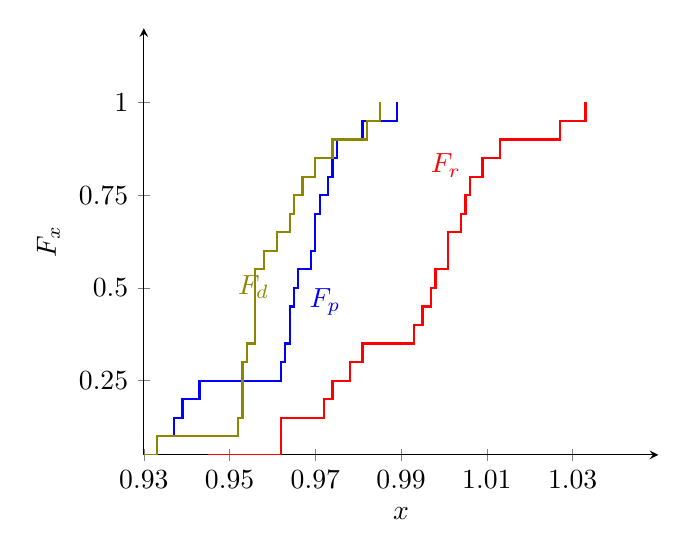
\begin{tikzpicture}
    \begin{axis}[%
        height=7cm,
        xlabel=$x$
        ,ylabel=$F_x$
        ,axis x line = bottom,axis y line = left
        ,ytick={0.25,0.5,...,1}
        ,ymax=1.2 % or enlarge y limits=upper
        ,xmin=0.93
        ,xmax=1.05
        ,xtick={0.91,0.93,...,1.02}
        ]
    \addplot+[red,const plot, no marks, thick] coordinates {(0.945, 0.050) (0.962, 0.100) (0.962, 0.150) (0.972, 0.200) (0.974, 0.250) (0.978, 0.300) (0.981, 0.350) (0.993, 0.400) (0.995, 0.450) (0.997, 0.500) (0.998, 0.550) (1.001, 0.600) (1.001, 0.650) (1.004, 0.700) (1.005, 0.750) (1.006, 0.800) (1.009, 0.850) (1.013, 0.900) (1.027, 0.950) (1.033, 1.000) } node[above=0.85cm, pos=.57,red] {$F_r$};
    
    \addplot+[blue,const plot, no marks, thick] coordinates {(0.931, 0.050) (0.933, 0.100) (0.937, 0.150) (0.939, 0.200) (0.943, 0.250) (0.962, 0.300) (0.963, 0.350) (0.964, 0.400) (0.964, 0.450) (0.965, 0.500) (0.966, 0.550) (0.969, 0.600) (0.970, 0.650) (0.970, 0.700) (0.971, 0.750) (0.973, 0.800) (0.974, 0.850) (0.975, 0.900) (0.981, 0.950) (0.989, 1.000)} node[below=1.2cm,pos=.77,blue] {$F_p$};
    
    \addplot+[olive,const plot, no marks, thick] coordinates {(0.927, 0.050) (0.933, 0.100) (0.952, 0.150) (0.953, 0.200) (0.953, 0.250) (0.953, 0.300) (0.954, 0.350) (0.956, 0.400) (0.956, 0.450) (0.956, 0.500) (0.956, 0.550) (0.958, 0.600) (0.961, 0.650) (0.964, 0.700) (0.965, 0.750) (0.967, 0.800) (0.970, 0.850) (0.974, 0.900) (0.982, 0.950) (0.985, 1.000)} node[above=0.25cm,pos=.36,olive] {$F_d$};
    \end{axis}
    \end{tikzpicture}
    }
  \caption{EDF of $\theta/\alpha$}
  \label{fig:sub2}
\end{subfigure}
\end{figure}


\begin{center}
\tiny
Source of the content: Gcinizwe Dlamini, Giancarlo Succi, Nataliya Tupikina ``Is the mind of a software developer similar to that of an artist? Focus on drawing,'' Under review, 2023.
\end{center}
\end{frame}

\begin{frame}
{\centerline{Processes in drawing and in software}}

\begin{itemize}
\item Iterative development
\item Customer orientation
\item Customer involvement
\item Pairing
\item Elimination of waste
\item Reuse
 \end{itemize}

\end{frame}


\begin{frame}
{\centerline{Incremental development -- 1}}

\begin{center}
\includegraphics[width=9cm]{P2023.AIBCCSS.Drawing/Leonardo.jpg}
\end{center}

\end{frame}

\begin{frame}
{\centerline{Incremental development -- 2}}

\begin{center}
\includegraphics[width=9cm]{P2023.AIBCCSS.Drawing/repin_sketch.jpg}
\end{center}

\end{frame}

\begin{frame}
{\centerline{Incremental development -- 3}}

\begin{figure}
\centering
\begin{subfigure}{.5\textwidth}
  \centering
  \includegraphics[width=.9\linewidth]{P2023.AIBCCSS.Drawing/sketch1.jpg}
\end{subfigure}%
\begin{subfigure}{.5\textwidth}
  \centering
  \includegraphics[width=.8\linewidth]{P2023.AIBCCSS.Drawing/sketch2.jpg}
\end{subfigure}
\end{figure}

\end{frame}


\begin{frame}
{\centerline{Incremental development -- 4}}

\begin{center}
\includegraphics[width=9cm]{P2023.AIBCCSS.Drawing/zasedanie.jpg}
\end{center}

\end{frame}





\begin{frame}
{\centerline{Customer orientation}}

\begin{center}
\includegraphics[width=8cm]{P2023.AIBCCSS.Drawing/serov_turchaninov.jpg}
\end{center}

\end{frame}

\begin{frame}
{\centerline{Customer involvement}}

\begin{figure}
\centering
\begin{subfigure}{.5\textwidth}
  \centering
  \includegraphics[width=.9\linewidth]{P2023.AIBCCSS.Drawing/yoko.jpg}
\end{subfigure}%
\begin{subfigure}{.5\textwidth}
  \centering
  \includegraphics[width=.8\linewidth]{P2023.AIBCCSS.Drawing/smoke.jpeg}
\end{subfigure}
\end{figure}

\end{frame}


\begin{frame}
{\centerline{Pair Painting -- 1}}

\begin{center}
Rubens and Breughel: Smell\\ 
\vspace{0.3cm}
\includegraphics[width=9cm]{P2023.AIBCCSS.Drawing/rub_and_br.jpg}
\end{center}

\end{frame}

\begin{frame}
{\centerline{Pair Painting -- 2}}

\begin{center}
Shishkin and Savitsky: Morning in a pine forest\\ 
\vspace{0.3cm}
\includegraphics[width=9cm]{P2023.AIBCCSS.Drawing/shish.jpg}
\end{center}

\end{frame}

\begin{frame}
{\centerline{Pair Painting -- 3}}

\begin{center}
Yakovlev and Shukhaev: Harlequin and Pierrot\\ 
\vspace{0.3cm}
\includegraphics[width=5cm]{P2023.AIBCCSS.Drawing/yakovlev.jpeg}
\end{center}

\end{frame}

\begin{frame}
{\centerline{Elimination of Waste}}

\begin{center}
\includegraphics[width=4.5cm]{P2023.AIBCCSS.Drawing/An_Anna_Blume.jpg}
\end{center}

\end{frame}

\begin{frame}
{\centerline{Reuse -- 1}}

\begin{figure}
\centering
\begin{subfigure}{.5\textwidth}
  \centering
  \includegraphics[width=0.95\linewidth]{P2023.AIBCCSS.Drawing/joy-of-life.jpg}
\end{subfigure}%
\begin{subfigure}{.5\textwidth}
  \centering
  \includegraphics[width=0.95\linewidth]{P2023.AIBCCSS.Drawing/dance.jpg}
\end{subfigure}
\end{figure}

\end{frame}

\begin{frame}
{\centerline{Reuse -- 2}}

\begin{figure}
\centering
\begin{subfigure}{.5\textwidth}
  \centering
  \includegraphics[width=0.95\linewidth]{P2023.AIBCCSS.Drawing/music1.jpg}
\end{subfigure}%
\begin{subfigure}{.5\textwidth}
  \centering
  \includegraphics[width=0.95\linewidth]{P2023.AIBCCSS.Drawing/music.jpg}
\end{subfigure}
\end{figure}

\end{frame}



\begin{frame}
{\centerline{Questions?}}
\vspace{1cm}
\begin{center}
    \LARGE{End of lecture seven.}
\end{center}

\end{frame}


\end{document}
